\chapter{Method}

At first, a heuristic criterion for temporal coherence between stream lines is defined.
Then ...


\begin{itemize}
    \item old implementation
    \item issues, why sth else was used
    \item turk and banks
    \item why turk and banks? (spacial coherence?)
    \item time coherence definition
\end{itemize}


\section{Temporal Coherence}
Temporal Coherence refers to how a vector field behaves through different time steps.
Intuitively, we consider areas within the field to be of high temporal coherence if the lines drawn on them are relatively stationary.
Vice versa, we can say that an area of high fluctuation will be of low temporal coherence.
A more formal definition employed in our algorithm is as follows:
Given a field $F$ and a starting point $S_0$ (called the "seed"), we can integrate over the field.
This yields a set of points $S^0$ which define a streamline containing every reached point, written as $S^0 = \int(S_0, F)$.
We can therefore assign a streamline to every point in our field (and vice versa).
Given $S_0$ and an unsteady field $F(t)$, compute for each time step $t_1...t_n$ the streamline $S^{0,t_i} = \int(S_0, F(t_i))$.
In order to convert these sets of lines to a scalar, we use the Hausdorff Distance $dist(S^i,S^j)$,
giving us the greatest minimal distance between any pair of two sets.
We can therefore create a map $coh(S_i, F(t)): max(dist(\int(S_i, F(t_k)), \int(S_i, F(t_l))))$,
sending each point in an unsteady vector field to a scalar, and thereby determining its temporal coherence.


\section{Technical details}
\subsection{Energy Measure}
The method used by Turk and Banks defines three important components to measure image quality as the sum of deviations of a low-pass image from a uniform greyscale target.
\begin{enumerate}
    \item The first component is a collection of (straight) line segments from each line,
    each of which can be converted to a line formula of the form $p = start + (end - start) * c$.
    The formula is then evaluated to obtain points as pixels where the low-pass filter in the 2nd listing is applied.
    In their paper, they call the implicit image obtained from the line segments' footprint $I$.
    \begin{equation*}
        I(x,y) = \begin{cases}
            1, \kern4em & \text{pixel lies on line}\\
            0,          & \text{else}
    \end{cases}
    \end{equation*}
    
    \item The second component is the low-pass filter $L$.
    It uses a kernel to generate the filtered image of a line.
    Given a falloff distance $R$ and $r=\sqrt{x^2+y^2} / R$, the kernel is defined as:
    \begin{equation*}
        K(x,y) = \begin{cases}
            2r^3 - 3r^2 + 1, \kern4em & r < 1\\
            0,               & r >= 1
        \end{cases}
    \end{equation*}
    For every pixel a line passes through, this kernel is applied additively, with its origin centered on the pixel containing the line.
    When applied consecutively along a line segment, the kernel will overlap and produce numbers from 1 to $2R$ for pixels close to the line.
    
    \item In order to determine the energy of the image generated by the kernel application, the following expression is used:
    \begin{equation*}
        E(I) = \int_x\int_y\left[(L\ast I)(x,y)-t\right]^2\,dx\,dy
    \end{equation*}
    With $t$ referring to the \textit{target brightness}, in their source code the number one is used.
\end{enumerate}

\noindent Our implementation works similarly, except that instead of the cubic Hermite filter, we use a two-dimensional Gauss filter.
We also use the distance $R$ as the radius of the filter, and calculate a small segment of a straight line in order to determine
how the brightness of the filter should be scaled to reach $1.5t$, so that we do not have to deal with differences depending on integration step size. 
More precisely, given the radius $R$ and filter diameter $D=2R+1$, we define a line footprint $A \in \mathbb{R}^{D\times D}$:
\begin{equation*}
    A_{x,y} = \begin{cases}
        1, \kern4em & x = R\\
        0, \kern4em & \text{otherwise}
    \end{cases}
\end{equation*}
We then apply our filter with $\sigma = R/3$, and use $1.5t  / A_{[R,R]}$ as our filter scale $s$, (in our case $t=1$).
Having obtained the filter scale, we can now compute the filtered image $L\ast I$ as $L\ast I = s \cdot Gauss(I, \sigma, R)$.
The computation of $E(I)$ is otherwise identical.

\subsection{Randomized Optimizations}
Turk and Banks define six actions:
\begin{itemize}
    \item \textbf{Insert, Delete:} Add or remove a line from the image.
    \item \textbf{Lengthen, Shorten:} In-/Decrease the length of a line on one or both ends.
    \item \textbf{Combine:} Join two lines head-to-tail.
    \item \textbf{Move:} Translate the seed of a line by a small distance.
\end{itemize}
These actions are selected randomly with random parameters, then applied to a random line.
The algorithm terminates after an energy range was reached, or accepted changes become rare enough to not introduce changes anymore.\\
\begin{minipage}{.55\textwidth}
    \vspace{5pt}
    If the change was deemed beneficial according to a decrease in energy, it is accepted, otherwise the changes are reverted.
    This causes a "drift" of the lines toward a more uniform energy level.
    Naturally, this depends heavily on the choice of $t$. If $t$ were to be chosen closer to 2,
    the image would become very crowded to reach the increased target gray level.
    \vspace{5pt}
\end{minipage}
\begin{minipage}{.45\textwidth}
    \begin{center}
        \includegraphics*{figures/SL_bump1.png}
        \captionof{figure}{A line (green) being shifted away from an existing one (black)}
    \end{center}
    \vspace*{5pt}
\end{minipage}
We have chosen to keep most of these actions as-is, the only difference introduced is
a change to how the lengthening and shortening is done. 
Instead of the two binary choices of lengthen/shorten and front/back, which only add/subtract a tiny bit at a time,
we decided to choose a segment count at random between -5 and 5 for each end.
This allows faster growth/shrinking (and hence faster convergence) while still preventing overlaps.

\subsection{Initial Seeding}
We prepare the image for the optimization routine by adding many streamlets with seeds on a regular grid to the image.
This can also be done randomly yielding similar image quality,
however strided access is more efficient with little to no benefit for the latter.

\subsection{Oracle}
The oracle from Turk and Bank's algorithm is used to suggest shorten/lengthen and move operations.
Our oracle focuses on shorten/lengthen suggestions only.

\subsection{Adding time coherence}
We added two important modifications to the aforementioned algorithm to make it partially time-coherent.
The first modification affects how seeds are chosen in the beginning of an optimization pass; the second affects
how the energy measure is computed and lines are guided toward their final positions.

\subsubsection*{Shattering}
At the end of a time step's optimization phase, we break every streamline apart into smaller streamlets.
This leaves each line with the appearance of simply being a dashed line, with each fragment having its own seed.
The seeds obtained this way are then used as the initial seeding strategy for the subsequent frame; the regular grid is only used for the first frame.
This way, we obtain many seeds that, if the field does not change too much, will quickly merge back into the line they came from.
If the field \textit{does} change, some segments will still reconnect and therefore keep their temporal coherence,
whereas areas of strong fluctuation will connect to different seeds.
This results in changes being limited to parts where change is necessary, and not affecting streamline trajectory too much on a global level.

\subsubsection*{Coaxing}
Since the energy function is used to move the image toward a constant desired target brightness, we achieve a uniform spacing of lines.
Unfortunately, this does not guarantee the lines be placed at similar positions as they were in the previous frame.
In order to coax the algorithm into favoring previous line positions, we modify $t$ to not be a constant anymore.
Instead, given the previous frame's $L$ (written $L'$) we replace $t$ with $T\in\mathbb{R}^{x\times y}$ defined as 
\begin{equation*}
    T_{x,y} = t + \left(L'_{x,y}\bigg|_0^{2t} - t\right) \cdot 0.4
\end{equation*}
The remaining operations stay the same, so our new energy expression becomes:
\[E(I, T) = \int_x\int_y\left[(L\ast I)(x,y)-T(x,y)\right]^2\,dx\,dy\]
This gives us some more fine-grained control of where lines will end up.
Due to the squishing of the typical $[0, \approx2t]$ domain of the last filtered image to only $[-.4t, .4t]$,
we soften the impact of the previous frame.
Otherwise, adding a line at the exact same position would only yield the target brightness,
causing a bunching of lines around these footprints.\\
\begin{minipage}{.5\textwidth}
    How does choosing the Gauss filter impact the ditches left by time coherence in the field? 
\end{minipage}
\begin{minipage}{.5\textwidth}
    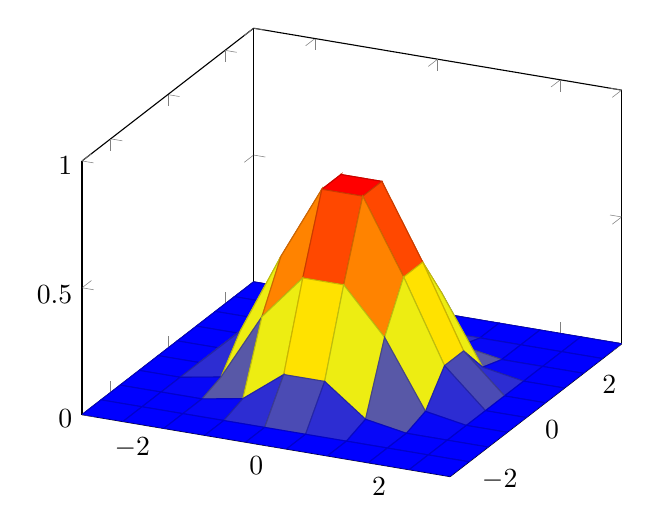
\begin{tikzpicture}[]
    \def\r(#1,#2){sqrt((#1)^2 + (#2)^2) / 2}
    \def\K(#1,#2){2 * \r(#1,#2)^3 - 3 * \r(#1,#2)^2 + 1}
    \begin{axis}[
        % xmin=-2.5,xmax=2,
        % ymin=-2.5,ymax=2,
        zmin= 0  ,zmax=1,
        % axis line style={draw=none},
        % axis equal image,
    ]
    \addplot3[
        surf,
        domain=-3:3,
        samples=10
    ]
    % K(x,y) = 2r^3 - 3r^2 + 1 if r < 1 else 0
    % r = sqrt(x^2 + y^2) / R
    % R = desired radius, lets use 2
    % therefore we get:
    % r = sqrt(x^2 + y^2) / 2
    % K(x,y) = sqrt(x^2 + y^2) / 2 < 1 ? 2 * (sqrt(x^2 + y^2) / 2) ^ 3 - 3 * (sqrt(x^2 + y^2) / 2) ^ 2 + 1 : 0
    {\r(x,y) < 1 ? \K(x,y) : 0};% < 1 ? 2 * r(x,y) ^ 3 - 3 * r(x,y) ^ 2 + 1 : 0};
    \end{axis}
\end{tikzpicture}
\pgfmathdeclarefunction{gauss}{1}{%
    \pgfmathparse{1/(#1*sqrt(2*pi))*exp(-(x^2)/(2*#1^2))}%
}
\pgfmathdeclarefunction{gauss2}{1}{%
    \pgfmathparse{1/(#1*sqrt(2*pi))*exp(-((x)^2 + (y)^2)/(2*#1^2))}%
}
\begin{tikzpicture}[]
    \begin{axis}[
        % xmin=-2.5,xmax=2,
        % ymin=-2.5,ymax=2,
        zmin= 0  ,zmax=1,
        % axis line style={draw=none},
        % axis equal image,
    ]
    \def\r(#1,#2){sqrt((#1)^2 + (#2)^2) / 2}
    \addplot3[
        surf,
        domain=-3:3,
        samples=40
    ]
    {\r(x,y) < 1 ? 1.6666 * gauss2(2/3) : 0};
    \end{axis}
\end{tikzpicture}
\begin{tikzpicture}
    \begin{axis}[every axis plot post/.append style={
        ultra thick, samples=100, domain=-2.5:2.5, mark=none}]
        \addplot {abs(x) < 2 ? 1.6666 * gauss(2/3) : 0};
        \def\r(#1){abs(#1) / 2}%
        \addplot[color=red, dotted]{
            \r(x) < 1 ? 2*(\r(x))^3-3*(\r(x))^2+1 : 0
        };
    \end{axis}
\end{tikzpicture}
\end{minipage}


\subsubsection*{Combined}
\begin{minipage}{.55\textwidth}
    Combining shattering and coaxing, we obtain a somewhat reliable way of generating streamlines according to the footprint left behind by the last frame.
    The seeds created during the shatter process all lie inside the "valley" left behind by the previous streamline path.
    Due to the coaxing function of the modified energy measure,
    it is unlikely that they will leave this valley without a change in the field forcing them to.
\end{minipage}
\begin{minipage}{.45\textwidth}
    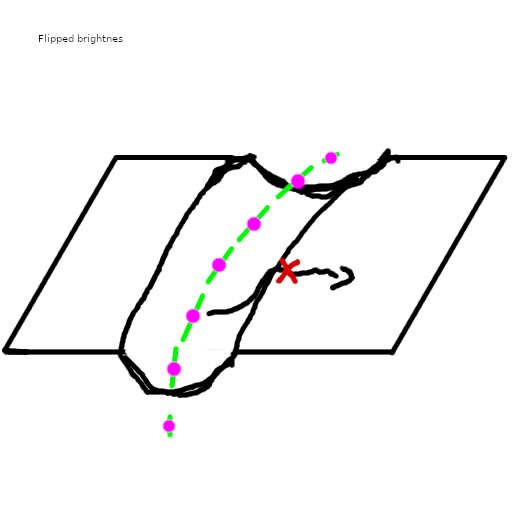
\includegraphics{figures/SL_bump2.png}
    \captionof{figure}{The Fragments' seeds (magenta) "trapped" inside the footprint of previous line}
\end{minipage}
Due to the seeds being held in place in this way, it is very likely for them to re-join to form the same lane they originated from.
If the field changes drastically in this region, the seeds can not fully connect to each other anymore, and will instead gravitate to a different footprint,
forming long patches of coherent lines with interconnections between different paths.
